\chapter{Spectral Pollution}
\section{Background}
In this document, we are going to investigate the spectral pollution in the problem
\begin{equation} \label{polynomial-eigenvalue-problem}
	\omega^2v + 2iv_0\dv{v}{x} + (1-v_0^2)\dv[2]{v}{x} = 0, \;\;\; v(\pm 1) = 0
\end{equation}

where the dispersion relation is known,
\begin{equation} \label{dispersion-relation}
	\omega = k(v_0 \pm 1) 
\end{equation}

If we introduce staggered grid, then there are 2 possible ways to discretize the Eq.(\ref{polynomial-eigenvalue-problem}).

\begin{figure}[H]
	\centering
	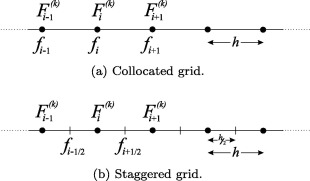
\includegraphics[width=0.7\linewidth]{img/staggered-grid.jpg}
\end{figure}

\begin{enumerate}
	\item Discretize the equation on the OPPOSITE grid where the function $v$ is defined on.
	\item Discretize the equation on the SAME grid where the function $v$ is defined on.
\end{enumerate}


If we assume $v\sim \exp(-ikx)$, and let $\beta\equiv kh/2$. Then the differential operators $\dv*[n]{x}$ are equivalent to the following factors \cite{llobet_spectral_1990},
\begin{itemize}
	\item Evaluate equation on the OPPOSITE grid
	align
	\begin{align}
		&H_0 = [\exp(i\beta)+\exp(-i\beta)]/2 = \cos(2\beta) \nonumber \\
		&H_1 = [\exp(i\beta)-\exp(-i\beta)]/h = (2i/h)\sin(\beta) 
		\label{H-operator} \\
		&H_2 = [\exp(3i\beta)-\exp(i\beta)-\exp(i\beta)+\exp(-3i\beta)]/2h^2 = H_1^2H_0 \nonumber 
	\end{align}
	
	\item Evaluate equation on the SAME grid
	\begin{align}
		&G_0 = 1 \nonumber \\
		&G_1 = [\exp(2i\beta)-\exp(-2i\beta)]/2h = (i/h)\sin(2\beta) = H_1H_0 
		\label{G-operator}\\
		&G_2 = [\exp(2i\beta)-2-\exp(-2i\beta)]/h^2 = (2/h^2)(\cos(2\beta)-1) = H_1^2 \nonumber 
	\end{align}
\end{itemize}


\section{Analysis of Numerical Spectrum}
\subsection{Discretize on the Same Grid}
Using the G-operator, Eq.(\ref{G-operator}), the discretized equation of Eq.(\ref{polynomial-eigenvalue-problem}) is 
\[ \omega^2 + \omega(2iv_0H_1H_0) + (1-v_0^2)H_1^2 = 0 \]

Thus the numerical dispersion relation is
\begin{equation} \label{dispersion-relation-G}
	\omega = -iH_1 \left(v_0 \pm \sqrt{v_0^2H_0^2 + (1-v_0^2)}\right) = \frac{2\sin(\beta)}{h}\left(v_0 \pm \sqrt{1 - v_0^2\sin[2](\beta)}\right)
\end{equation}

We see that 
\begin{itemize}
	\item $\omega$ is real for all $k$ if $v_0 < 1$.
	\item $\omega$ is complex for large $k$, more specifically $k>h/2\arcsin(1/v_0)$, if $v_0 > 1$.
	\item For small $k$, meaning $k\to 0$, Eq.(\ref{dispersion-relation-G}) is a good representation for the analytical dispersion relation, Eq.(\ref{dispersion-relation}). 
\end{itemize}
This explains why the spurious unstable modes occur when $v_0>1$.


\begin{figure}[H]
	\centering
	\begin{subfigure}[b]{0.5\linewidth}
		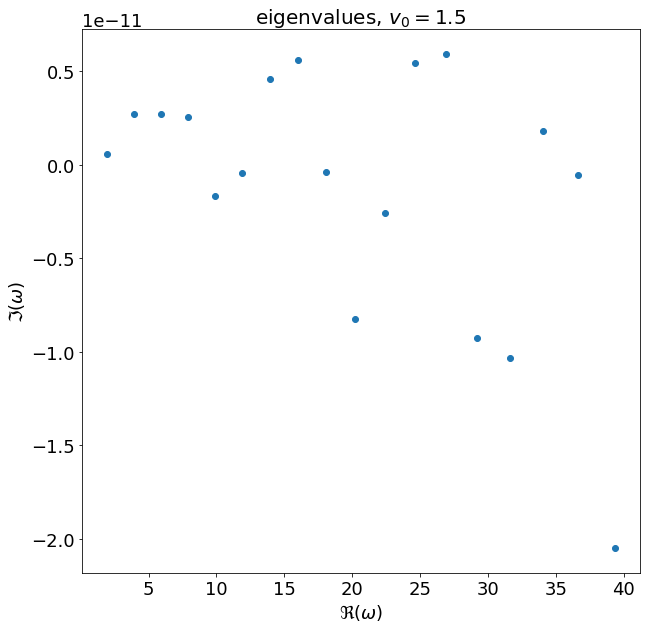
\includegraphics[width=\linewidth]{img/eigvals-G-filtered.png} 
		\caption{Filtered eigenvalues}
		\label{fig:results-G-a}
	\end{subfigure}%
	\begin{subfigure}[b]{0.5\linewidth}
		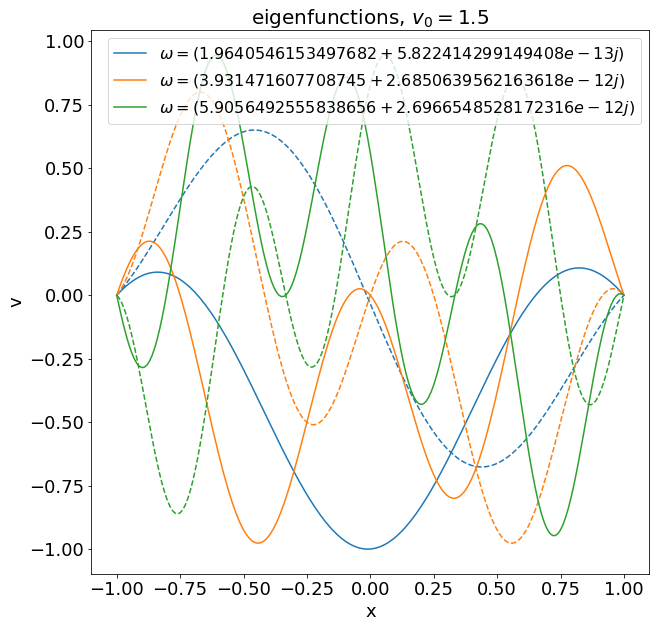
\includegraphics[width=\linewidth]{img/eigfuncs-G-filtered.png} 
		\caption{Filtered eigenfunctions}
		\label{fig:results-G-b}
	\end{subfigure}
	\caption{Filter out the spurious modes with $k>h/2\arcsin(1/v_0)$.}
	\label{fig:results-G}
\end{figure}

\subsection{Discretize on the Opposite Grid}
Using the H-operator, Eq.(\ref{H-operator}), Eq.(\ref{polynomial-eigenvalue-problem}) becomes
\[ \omega^2H_0 + \omega(2iv_0H_1) + (1-v_0^2)H_1^2H_0 = 0 \]

So the numerical dispersion relation is
\begin{equation}\label{dispersion-relation-H}
	\omega = -iH_1 \left(v_0 \pm \sqrt{v_0^2 + (1-v_0^2)H_0^2}\right) = \frac{2\sin(\beta)}{h}\left(v_0 \pm \sqrt{\cos[2](\beta) + v_0^2\sin[2](\beta)}\right)
\end{equation}

We see that 
\begin{itemize}
	\item $\omega$ is real for all $k$ for all $v_0$.
	\item For small $k$, Eq.(\ref{dispersion-relation-H}) dramatically deviates from the analytical dispersion relation Eq.(\ref{dispersion-relation}). 
\end{itemize}

\begin{figure}[H]
	\centering
	\begin{subfigure}[b]{0.3\linewidth}
		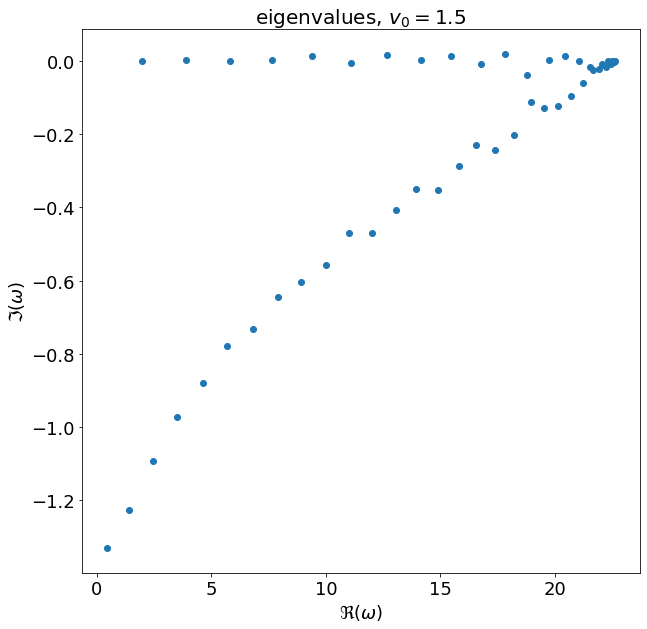
\includegraphics[width=\linewidth]{img/eigvals-H.png} 
		\caption{Deformed eigenvalues, accumulation point occurs.}
		\label{fig:results-H-a}
	\end{subfigure}
	\begin{subfigure}[b]{0.3\linewidth}
		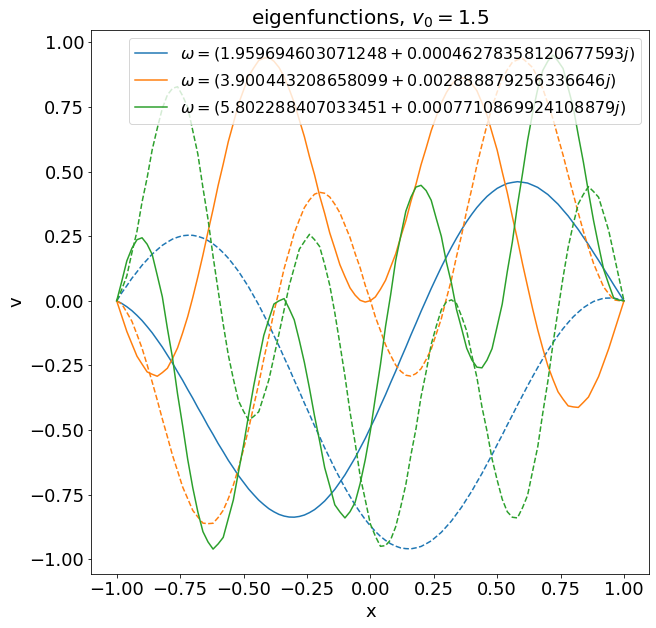
\includegraphics[width=\linewidth]{img/eigfuncs-good-H.png} 
		\caption{Good eigenfunctions}
		\label{fig:results-H-b}
	\end{subfigure}
	\begin{subfigure}[b]{0.3\linewidth}
		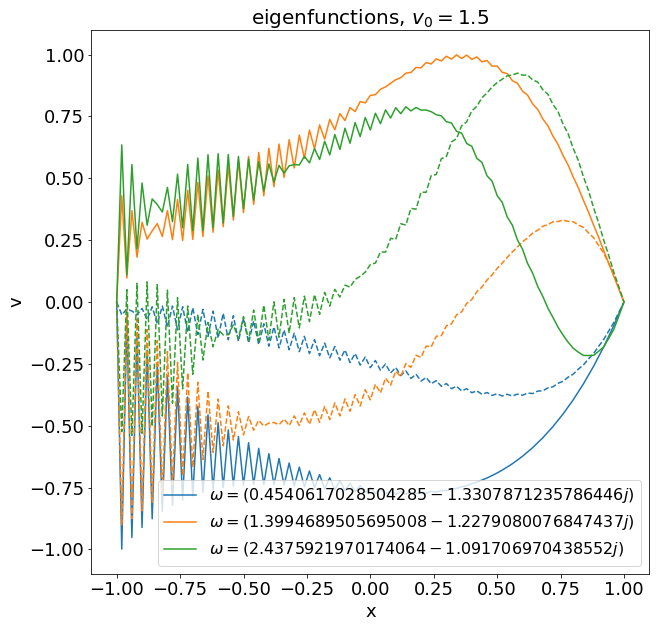
\includegraphics[width=\linewidth]{img/eigfuncs-bad-H.png}
		\caption{Spurious modes.} 
		\label{fig:results-H-c}  
	\end{subfigure}
	\caption{Although the spurious unstable modes are much smaller, but the eigenvalues deviate from the analytical dispersion relation.}
	\label{fig:results-H}
\end{figure}

\section{Conclusion}
\begin{enumerate}
	\item If we discretize Eq.(\ref{polynomial-eigenvalue-problem}) on the same grid as the function $v$ is defined on, then the eigenvalues are good for small $k$ modes. To get the good modes, we can filter out the modes with wave number $k>h/2\arcsin(1/v_0)$.
	\item While we get less spurious unstable modes if we discretize Eq.(\ref{polynomial-eigenvalue-problem}) on the opposite grid as the $v$ is defined on, we suffer the inaccurate eigenvalues.
\end{enumerate}